\documentclass[standalone, version=2.0]{huangfusl-template}
\begin{document}
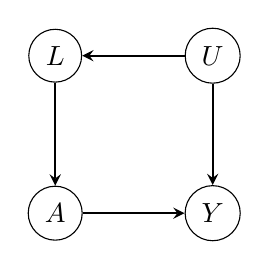
\begin{tikzpicture}
    \node[circle, draw] (L) at (-1, 1) {$L$};
    \node[circle, draw] (U) at (1, 1) {$U$};
    \node[circle, draw] (A) at (-1, -1) {$A$};
    \node[circle, draw] (Y) at (1, -1) {$Y$};

    \draw[-stealth, thick] (L) -- (A);
    \draw[-stealth, thick] (U) -- (Y);
    \draw[-stealth, thick] (A) -- (Y);
    \draw[-stealth, thick] (U) -- (L);
\end{tikzpicture}
\newpage
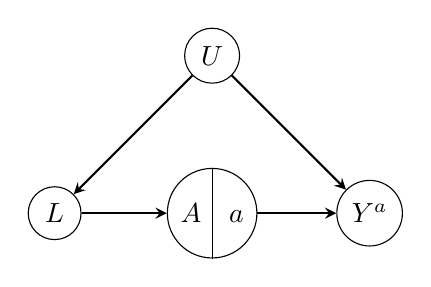
\begin{tikzpicture}
    \node[circle, draw] (L) at (-3, -1) {$L$};
    \node[circle, draw] (U) at (-1, 1) {$U$};
    \node[circle, draw] (A) at (-1, -1) {$A \quad a$};
    \node[circle, draw] (Y) at (1, -1) {$Y^a$};

    \draw[-stealth, thick] (L) -- (A);
    \draw[-stealth, thick] (U) -- (Y);
    \draw[-stealth, thick] (A) -- (Y);
    \draw[-stealth, thick] (U) -- (L);
    \draw (A.north) -- (A.south);
\end{tikzpicture}
\end{document}